\chapter{Defining the general use cases}
\label{ch:usecases}

\section{Supplantive or generative}

The first important design choice which has to be made is whether the students are supplied with a concept map or flashcards, or that they generate the content themselves. The dichotomy of generative versus supplantive instruction is described in further detail by \citeA{instructionaldesign}, where the implications of both sides are enlisted for the learner, the task and the context.

One of the aspects of generative strategies is that the learner requires a higher amount of prior knowledge, a higher aptitude, and a wider and more flexible range of cognitive strategies, because the content still has to be (partly) researched and constructed. This can be a disadvantage, because the learner might not possess these skills and therefore the instruction may not be suitable or highly inefficient using generative strategies. On the other hand, greater mental effort generally leads to greater depth of processing and therefore better, more meaningful learning, which was also stressed by \citeA{canas} and \citeA{nesbit}. Furthermore, learners experience a higher motivation and a lower amount of anxiety when using generative strategies, and their attribution of success is internal rather than external. 

Furthermore, when using more generative strategies, the learning task becomes more complex and ill-structured, and therefore requires more instruction and time to complete. It also leads to a higher focus on cognitive strategies, but less so on the learning goals. These goals can also not become universal, since each student creates their own flashcards or concept map, and therefore decides on their own learning content.

The most important factor for this design choice is feasibility. The teacher already stated that there is only limited time available during the lesson to introduce them to the software, so there is no time for extensive instruction on how to create concept maps, let alone creating the maps within the classroom. Additionally, students do not have much time at home to spend on creating the maps, and it is also known from both interviews with the teacher as literature that they will probably have only a low amount of intrinsic motivation. Finally, when the students have to create their own maps, it cannot be guaranted that they will include the nodes relevant for the goals of the instruction, and might become either to narrow or to extensive in certain branches. The same arguments are valid for letting students create their own flashcards. Therefore, despite of the benefits that a more generative approach may have for the learning process, the content will be supplied to the students instead.

\section{Supported user actions}

The other design decision related to the general ideation of software is deciding which use cases should be supported, which are typically displayed within UML use case diagrams \cite{uml}. For the flashmap software, the use cases are divided in cases related to the registering and login process (see figure~\ref{fig:loginusecase}), and the cases related to the main use of the software (see figure~\ref{fig:mainusecase}).

\begin{figure}[h!]
\centering
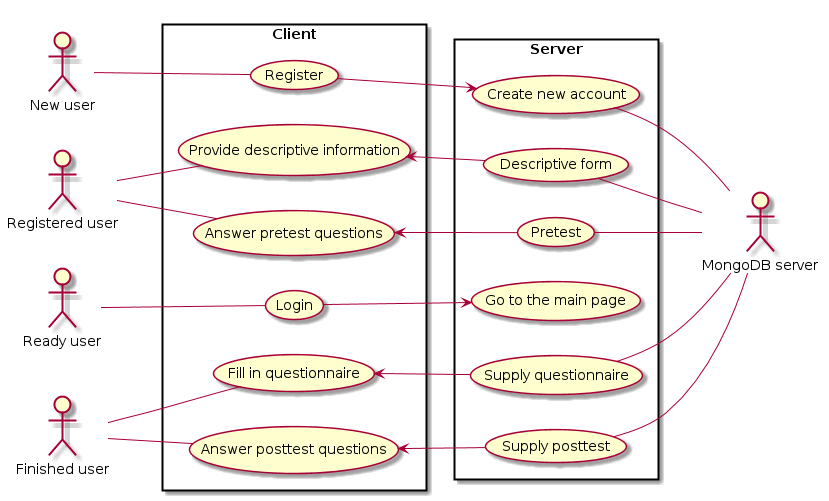
\includegraphics[width=\textwidth]{img/loginusecase.png}
\caption{An UML use case diagram for registering as new users or logging in as existing users}
\label{fig:loginusecase}
\end{figure}

\paragraph{Login use cases} When opening the webapplication, the user is first prompted with a login screen. Here, the user can either enter an already existing username to continue this session, or he can enter a new name in order to register as a new user. When the user is registering as a new user, a form is presented asking for information on gender and birthdate as descriptive information, and asking for the specific code the user received on the informed consent form in order to validate that the user indeed signed this form before partaking in the research (see section \nameref{sec:procedure} on page~\pageref{sec:procedure}). After that, another form will be prompted for the pretest (section \nameref{sec:instrumentation} on page~\pageref{sec:instrumentation}). When the user has met certain criteria, a posttest similar to the pretest will be prompted, followed by a questionnaire and a debriefing text. When none of these criteria are met, the user can access he main use cases.

\begin{figure}[h!]
\centering
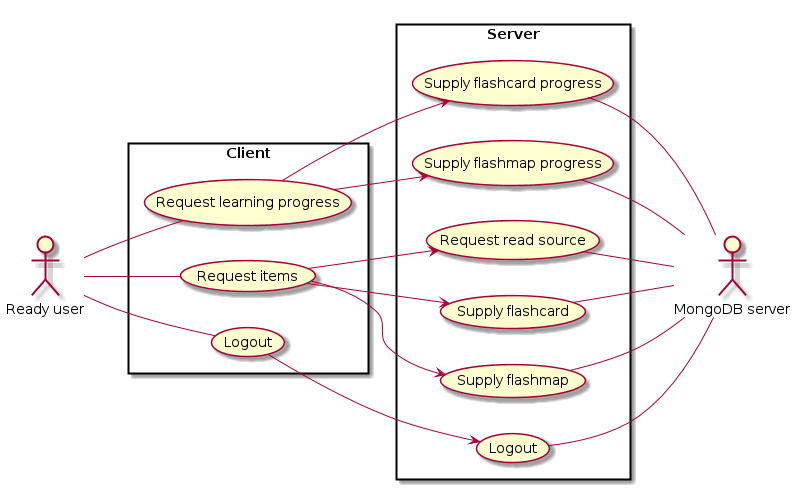
\includegraphics[width=\textwidth]{img/mainusecase.png}
\caption{An UML use case diagram for main uses of the application}
\label{fig:mainusecase}
\end{figure}

\paragraph{Learning use cases} The main use cases entail requesting items for review, requesting the learning progress, or logging out. When requesting items for review, the user can receive a due or new flashcard or flashmap, depending whether there are any old items due for review and the experimental group the user is in. Alternatively, the user can also be prompted whether a certain section of the instruction material has been read, since the rehearsal of items cannot be meaningful when the user is not familiar with the content. These prompts take often place at the beginning of a session so that the user does not have to interrupt a session. Furthermore, they prompt two sections ahead of the material currently being learned or reviewed by the user from the flashmap or flashcards in order to guarantee that the user is familiar with the material before learning the items. The user is prompted to read a section at most once per day. After the user has submitted a response, he can undo this response if he is not content with it. For example, the user could after seeing the correct response decide that he thought of a similar enough answer, but after deeper reflection still decide that his answer was not sufficient. In this case, he could use the undo option in order to be presented with the previous response again and select the 'incorrect' option.

\paragraph{Learning progress} When requesting the learning progress, the user is presented of an overview of what has already been learned and what is still left as either unseen items or items due for review. This provides an indication for the user so that he can estimate how much time he still needs to invest into the software, but also could stimulate the user by seeing the number of new or due items lowering and learned items increasing.

Finally, the user can return to the login screen by logging out.
